\documentclass[a4paper,11pt]{article}
\usepackage[dvipdfmx]{graphicx}

\usepackage{here}
\begin{document}
\title{Smartcab}
\author{Ryosuke Honda}
\date{2016/06/23}
\maketitle




%%Section1
\section{Implement a basic driving agent}
\ \ \ \ Implement the basic driving agent, which processes the following inputs at each time step:
\begin{itemize}
\item Next waypoint location, relative to its current location and heading.
\item Intersection state(traffic light and presence of cars) and
\item Current deadline value(time steps remining)
\end{itemize}

And produces some random move/action [None,'forward','left','right'].
The rule and the reward of the agent are following.

\begin{itemize}
\item The start and goal location changes in each episodes.
\item When the car violates the traffic rule, the agent will get the negative reward(-1).
\item If the car moves without violating the traffic rule but the agent doesn't follow the waypoint,the agent will lose 0.5 points.
\item When the car moves without violating the traffic rule and follows the waypoint, the agent will get 2 reward points
\item When the car gets to the destination within the deadline, the agent will get 10 reward points.
\item When reaching goal within the deadline, the agent will always get 10 reward points, which means that reaching the destination doesn't always get the maximum reward for each episode.
 
\end{itemize}






%%Section2
\section{Identify and update state}

\ \ \ \ The agent can sense the information of inputs of traffic light, oncoming car, turning right and turning left which all of other agents have and what's more the agent has the information of next waypoint.
Since the start point and destination point will differ from each episode, it's not good to keep track of their points to get high rewards.
We should restore the information that keeps the same as the episode changes. Therefore, we should keep track of the traffic information which is traffic light, oncoming car,right and left. 
\par Those are the information which can sense the other agents can sense. The agent should keep the memory of waypoint. These information is necessary not to violate the traffic rules and to get high rewards.

As explained above, the Q table for this questions will be like this.

\begin{table}[H]
\begin{center}
\caption{Q table}
\begin{tabular}{|c|c|r|} \hline
States & Values & Dimentions  \\ \hline
Traffic light & Red &2 \\ 
 & Blue & \\ \hline
 & None & \\
Waypoint &Forward &4\\
 &Left &\\
 & Right &\\ \hline
 & None & \\
 Oncoming&Forward &4\\
 &Left &\\
 & Right &\\ \hline
 & None & \\
 Left&Forward &4\\
 &Left &\\
 & Right &\\ \hline
 & None & \\
Right &Forward &4\\
 &Left &\\
 & Right &\\ \hline

\end{tabular}
\end{center}
\end{table}

The possible action for the agent is "None","Forward","Right","Left"
The dimension of the q table is 2$\times$4$\times$4$\times$4$\times$4=512.




\section{Implement Q-learning}
\ \ \ \ One of the most important breakthroughs in reinforcement learning was the development of Q-learning.Its simplest form,one step Q-learning, is defined by

\begin{equation}
	Q(s,a)\leftarrow (1-\alpha)Q(s,a)+\alpha(r(s,a)+\gamma \max_{a'}(Q'(s',a')))
\end{equation}
$\alpha$:Learning rate $\gamma$:Discount rate \\
{\bf s}:state, {\bf a}:action, {\bf s'}:next state, {\bf a'}:all actions


First, set the parameters($\alpha$,$\gamma$) and environmental reward.Then Initialize the Q table to zero. For each episode, select a random initial state and do the following things until the agent has reached the goal.
\begin{itemize}
\item Select one among all possible actions for the current state.
\item Using this possible action, consider going to the next state.
\item Get maximum Q value for this next state based on all possible actions
\item Compute Q value
\item Set the next state as the current state
\end{itemize}


The gamma and alpha parameters has a range of 0 to 1. If gamma is closer to zero, the agent will tend to consider only immediate rewards. If alpha is closer to zero, the agent will tend to consider only past experience(don't learn).

Here, I introduce the code snippet of the $\epsilon$-greedy Q learning.
\begin{figure}[H]
\begin{center}
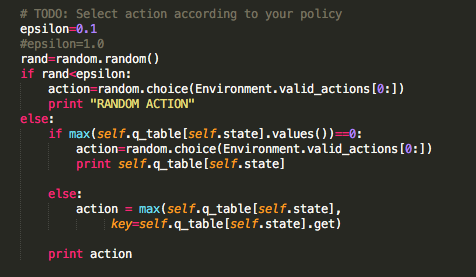
\includegraphics[width=100mm]{graph/python_code.jpg}
\end{center}
\caption{Python code snippet for deciding action policy}
\label{fig:1}
\end{figure}

In this experiment, I use $\epsilon$-greedy  and set $\epsilon$ to be 0.1. The agent chooses random action with the probability of 0.1. If the maximum of q-table is 0, the agent also chooses random action. If the maximum q-table is more than 0, the agent chooses the maximum value and moves toward it.


\begin{figure}[H]
\begin{center}
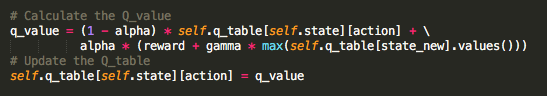
\includegraphics[width=100mm]{graph/python_code2.jpg}
\end{center}
\caption{Python code snippet for updating Q table}
\label{fig:2}
\end{figure}
The code above is the calculation of fomula(1) and code snippet for updating Q table.
I'll discuss the agent's behavior in the next section.








\section{Enhance the driving agent}
\ \ \ \ When the agent just started, it has no q-value since the q-table is set to be 0. Therefore, at first I need to set the move randomly($\epsilon$-greedy).
With the probability of $\epsilon$, the agent moves randomly. This prevents the agent from falling into the wrong choice. 
\\


%%Explanation for the First implementation
(I) First, I implemented random action.The agent just moves random action("None","Forward","Left","Right") and doesn't learn anything from experience.
\\
In the agent.py file, I set $\epsilon$ to be 1(The agents moves randomly).
I define "Success Rate" to see the agent's performance.


{\bf "Success Rate"="No.trials achieve goal before deadline" $\div$"No. trials"}



For these trials, the number of trials are 100.
In this experiment,I set the conditions as follows.


Success rate in this trial is 0.20.



        


\begin{figure}[H]
\begin{center}
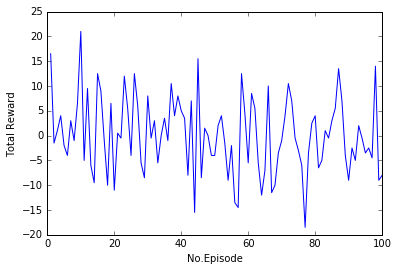
\includegraphics[width=100mm]{graph/random.jpg}
\end{center}
\caption{Random Action}
\label{fig:one}
\end{figure}

As the Fig\ref{fig:one} shows,the total rewards with this trial contains negative values.
Without learning from their experience, the agent won't get high reward.
\\

%%Explanation for the Second Implementation

(I\hspace{-.1em}I) Second, the parameters of $\alpha$ and $\gamma$ are 0.5 and 0.9 respectively.
With this condition, the success rate is 0.72 which is higher than the random action.

\begin{figure}[H]
\begin{center}
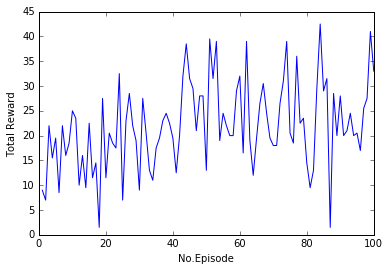
\includegraphics[width=100mm]{graph/constant.jpg}
\end{center}
\caption{Constant $\alpha$ and $\gamma$}
\label{fig:two}
\end{figure}

The Fig\ref{fig:two} shows,the total rewards for each episode are all positive and the cumulative sum of total reward of all episodes are 2195.5.
\\


%%Explanation for the Third Implementation
(I\hspace{-.1em}I\hspace{-.1em}I) Third, the parameters of $\alpha$ and $\gamma$ are as follows.

\begin{equation}
	\alpha=\frac{1.0}{1.0+time}
\end{equation}

\begin{equation}
	\gamma=\frac{1.0}{1.0+deadline}
\end{equation}

With this condition, the success rate is 0.86 which is higher than the trials before.


\begin{figure}[H]
\begin{center}
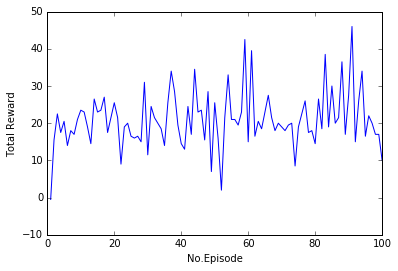
\includegraphics[width=100mm]{graph/better.jpg}
\end{center}
\caption{Fig}
\label{fig:three}
\end{figure}

The Fig\ref{fig:three} shows,the total rewards for each episode are all positive and the cumulative sum of total reward of all episodes are 2099.0
\\

%%Explanation for the Final Implementation
(I\hspace{-.1em}V) Final version

The condition in this implementation is as follows.
$\alpha$ is equal to the fomula (2) and $\gamma$ sets to be 0.9.

With this condition, the success rate is 0.86 which is the same value as the trial 3.

\begin{figure}[H]
\begin{center}
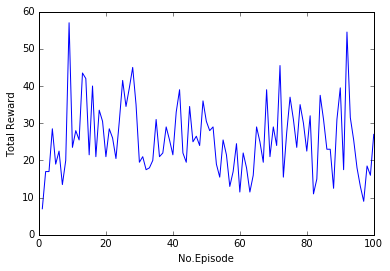
\includegraphics[width=100mm]{graph/gamma_con.jpg}
\end{center}
\caption{Fig}
\label{fig:four}
\end{figure}

The Fig\ref{fig:four} shows,the total rewards for each episode are all positive and the cumulative sum of total reward of all episodes are 2580.5.
The cumulative sum of total reward of all episodes are conspicuously higher than the other trials. 


\end{document}